\documentclass[letterpaper]{article}
\usepackage[margin=1in]{geometry}
\usepackage[utf8]{inputenc}
\usepackage{textcomp}
\usepackage{amssymb}
\usepackage{natbib}
\usepackage{graphicx}
\usepackage{gensymb}
\usepackage{amsthm, amsmath, mathtools}
\usepackage[dvipsnames]{xcolor}
\usepackage{enumerate}
\usepackage{mdframed}
\usepackage[most]{tcolorbox}
\usepackage{csquotes}
% https://tex.stackexchange.com/questions/13506/how-to-continue-the-framed-text-box-on-multiple-pages

\tcbuselibrary{theorems}

\newcommand{\R}{\mathbb{R}}
\newcommand{\Z}{\mathbb{Z}}
\newcommand{\N}{\mathbb{N}}
\newcommand{\Q}{\mathbb{Q}}
\newcommand{\C}{\mathbb{C}}
\newcommand{\code}[1]{\texttt{#1}}
\newcommand{\mdiamond}{$\diamondsuit$}
\newcommand{\PowerSet}{\mathcal{P}}
\newcommand{\Mod}[1]{\ (\mathrm{mod}\ #1)}
\DeclareMathOperator{\lcm}{lcm}

%\newtheorem*{theorem}{Theorem}
%\newtheorem*{definition}{Definition}
%\newtheorem*{corollary}{Corollary}
%\newtheorem*{lemma}{Lemma}
\newtheorem*{proposition}{Proposition}


\newtcbtheorem[number within=section]{theorem}{Theorem}
{colback=green!5,colframe=green!35!black,fonttitle=\bfseries}{th}

\newtcbtheorem[number within=section]{definition}{Definition}
{colback=blue!5,colframe=blue!35!black,fonttitle=\bfseries}{def}

\newtcbtheorem[number within=section]{corollary}{Corollary}
{colback=yellow!5,colframe=yellow!35!black,fonttitle=\bfseries}{cor}

\newtcbtheorem[number within=section]{lemma}{Lemma}
{colback=red!5,colframe=red!35!black,fonttitle=\bfseries}{lem}

\newtcbtheorem[number within=section]{example}{Example}
{colback=white!5,colframe=white!35!black,fonttitle=\bfseries}{def}

\newtcbtheorem[number within=section]{note}{Important Note}{
        enhanced,
        sharp corners,
        attach boxed title to top left={
            xshift=-1mm,
            yshift=-5mm,
            yshifttext=-1mm
        },
        top=1.5em,
        colback=white,
        colframe=black,
        fonttitle=\bfseries,
        boxed title style={
            sharp corners,
            size=small,
            colback=red!75!black,
            colframe=red!75!black,
        } 
    }{impnote}
\usepackage[utf8]{inputenc}
\usepackage[english]{babel}
\usepackage{fancyhdr}
\usepackage[hidelinks]{hyperref}

\pagestyle{fancy}
\fancyhf{}
\rhead{CSE 101}
\chead{Wednesday, January 05, 2022}
\lhead{Lecture 2}
\rfoot{\thepage}

\setlength{\parindent}{0pt}

\begin{document}

\section{Levels of Algorithm Design}
\begin{itemize}
    \item \textbf{Naive Algorithms:} Turn definition into algorithm. This is easy to wirte, good first pass, but often very slow. Good way to ``test.''
    \item \textbf{Toolkit:} Algorithms designed using standard tools the main focus of this course. 
    \item \textbf{Optimized:} Use data structures or other ideas to make algorithm especially efficient. 
    \item \textbf{Magic:} Sometimes, an algorithm requires a surprising new insight. 
\end{itemize}

\section{Graph}
\begin{definition}{Graph}{}
    A \textbf{graph} $G = (V, E)$ consists of two things:
    \begin{itemize}
        \item A collection $V$ of vertices, or objects to be connected.
        \item A collection $E$ of edges, each of which connects a pair of vertices.
    \end{itemize}
\end{definition}

For example, we can model the following as graphs: 
\begin{itemize}
    \item The internet, where $V$ is the websites and $E$ are links. 
    \item The internet, where $V$ are computers and $E$ are physical connections. 
    \item A highway system, where $V$ are the intersections and $E$ are the roads. 
\end{itemize}

\subsection{Examples of Graphs in CS}
In computer science, there are a few examples of graphs: 
\begin{itemize}
    \item The internet (webpages, physical connections, etc.)
    \item Social networks (especially with friendship, connections).
    \item Transitions between states of a program. 
    \item Road maps. 
\end{itemize}

\subsection{Drawing Graphs}
When drawing graphs, we want to draw the vertices first. Then, for each edge, draw line segments or curves connecting those points. 
\begin{center}
    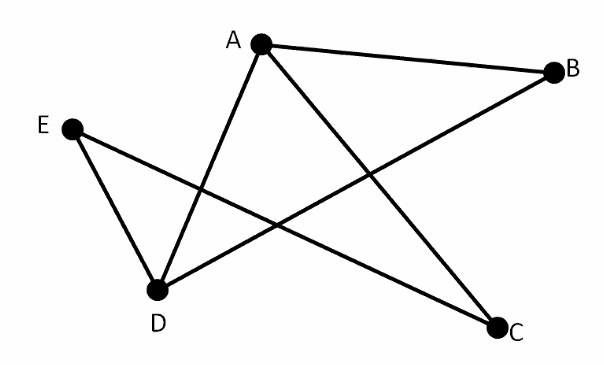
\includegraphics[scale=0.5]{../assets/graph.png}
\end{center}
This particular graph can be represented by $G = (V, E)$ where: 
\[V = \{A, B, C, D, E\}\]
\[E = \{(A, B), (A, C), (A, D), (B, D), (C, E), (D, E)\}\]
Because this is an \underline{unordered} graph, $(A, B)$ and $(B, A)$ mean the same thing. 

\subsection{Exploring Graphs}
Suppose we are playing a video game and want to make sure that you've found all the areas in this level before moving on to the next one. How do we ensure that we found everything? 

\subsubsection{Basic Algorithm}
Essentially, we want to: 
\begin{verbatim}
    Keep track of all areas discovered.
    While there is an unexplored path:
        Follow path. 
\end{verbatim}

\subsubsection{Systematize}
Essentially, we need to keep track of: 
\begin{itemize}
    \item Which vertices we have discovered. 
    \item Which edges have yet to be explored.
\end{itemize}
So, the explore algorithm will:
\begin{itemize}
    \item Use a field \code{v.visted} to let us know which vertices we have seen.
    \item Store edges to be explored implicitly in the program stack. 
\end{itemize}

\begin{verbatim}
    explore(v):
        v.visited <- true 
        for each edge (v, w):
            if not w.visited:
                explore(w)
                w.prev <- v     // If we want to keep track of path taken
\end{verbatim}

\subsubsection{Result}
\begin{theorem}{}{}
    If all vertices start unvisited, \code{explore(v)} marks as visited exactly the vertices reachable from \code{v}.
\end{theorem}

\begin{mdframed}[]
    \begin{proof}
        First, we note that we can only visit vertices that are reachable from $v$. If $u$ is visited, then eventally we will visit every adjacent $w$. If there is a chain of vertices, then $v$ will visit $u_1$ which will visit $u_2$ which will visit everything up to and including $w$. 
    \end{proof}
\end{mdframed}

\subsection{Depth First Search}
\code{explore} only finds the part of the graph reachable from a single vertex. If you want to discover the entire graph, you may need to run it multiple times. This introduces an algorithm known as \textbf{depth first search}:
\begin{verbatim}
    DepthFirstSearch(v):
        Mark all v in G as unvisited. 
        For v in G:
            if not v.visited:
                explore(v)
\end{verbatim}
Here, this runs in $O(|V|)$ time: we need to iterate over vertex. 

\subsection{Runtime of DFS}
\begin{verbatim}
    explore(v):                 // Run once per vertex O(|V|) 
        v.visited <- true       // Run once per vertex 
        for each edge (v, w):   // Run once per neighboring vertex O(|E|)
            if not w.visited:   // Run once per neighboring vertex
                explore(w)      // Run once per neighboring vertex
                w.prev <- v     // Run once per neighboring vertex
\end{verbatim}
So, our final runtime is: 
\[O(2|V| + |E|) = O(|V| + |E|)\]

\end{document}